\chapter{Ensembles on Random Patches}\label{ch:random-patches}

% sampling samples: an easy way to reduce time complexity
% sampling features: an easy way to decorrelate predictions

\begin{remark}{Outline}
In this chapter, we consider supervised learning under the assumption that the
available memory is small compared to the size of the dataset. This general framework
is relevant in the context of big data, distributed databases and embedded
systems. In Section~\ref{sec:9:rp}, we propose a very simple, yet effective,
ensemble framework that builds each individual model of the ensemble from a
random patch of data obtained by drawing random subsets of \textit{both}
samples and input variables from the whole dataset. In
sections~\ref{sec:9:accuracy} and \ref{sec:9:memory}, we carry out an extensive
and systematic evaluation of this method on 29 datasets, using decision trees
as base models. With respect to popular ensemble methods, these experiments
show that the proposed method provides on par  performance  in terms of
accuracy while simultaneously lowering the memory needs, and attains
significantly better performance when memory is severely constrained. We
conclude and discuss future work directions in Section~\ref{sec:9:conclusions}.
\textit{This chapter is based on previous work published in \citep{louppe:2012}.}
\end{remark}

Within the past few years, big data has become a popular trend among many
scientific fields. In life sciences, computer vision, Internet search or
finance, to cite a few, quantities of data have grown so large that it is
increasingly difficult to process, analyze or visualize. In many cases, single
computers are no longer fit for big data and distributed environments need to
be considered to handle it. Although research is very active in this area,
machine learning is no exception to this new paradigm. Much still needs to be
done and methods and algorithms have to be reinvented to take this constraint
into account.

In this context, we consider supervised learning problems for which the dataset
is so large that it cannot be loaded into memory. In~\citep{breiman:1999},
Breiman proposed the Pasting method to tackle this problem by learning an
ensemble of models individually built on random subsets of the training
examples, hence alleviating the memory requirements since the base models would
be built on only small parts of the whole dataset. Earlier, Ho proposed
in~\citep{ho:1998} to learn an ensemble of models individually built on random
subspaces (i.e., on random subsets of the features). While the first motivation
of the Random Subspace method was to increase the diversity within the models
of the ensemble, it can actually also be seen as way to reduce the memory
requirements of building individual models. In this work, we propose to combine
and leverage both approaches at the same time: learn an ensemble of models on
\textit{random patches}, i.e., on random subsets of the samples \textit{and} of
the input variables. Through an extensive empirical study, we show that this
approach (1) improves or preserves comparable accuracy with respect to other
ensemble approaches which build base models on the whole dataset while (2)
drastically lowering the memory requirements and hence allowing an equivalent
reduction of the global computing time.

\section{Random Patches}
\label{sec:9:rp}

The Random Patches algorithm proposed in this work (further referred to as RP)
is a wrapper ensemble method that can be described in the following terms. Let
${\cal R}(\alpha_s, \alpha_f, {\cal L})$ be the set of all random patches of
size $\alpha_s N \times \alpha_f p$ than can be drawn from the dataset ${\cal
L}$, where $N$ (resp., $p$) is the number of samples in ${\cal L}$ (resp.,  the
number of input variables in ${\cal L}$) and where $\alpha_s \in [0, 1]$ (resp.
$\alpha_f$) is an hyper-parameter that controls the number of samples in a
patch (resp., the number of variables). That is, ${\cal R}(\alpha_s, \alpha_f,
{\cal L})$ is the set of all possible subsets containing $\alpha_s N$ samples
(among $N$) with $\alpha_f p$ variables (among $p$). The method then works as
follows:

\begin{algorithm}\label{algo:rp}
Random Patches algorithm.
\textnormal{
\begin{algorithmic}[1]
    \For{$m=1, \dots, M$}
        \State Draw a patch $r \sim U({\cal R}(\alpha_s, \alpha_f, {\cal L}))$ uniformly at random
        \State Build a model on the selected patch $r$
    \EndFor
    \State Aggregate the predictions of the $M$ models in an ensemble
\end{algorithmic}
}
\end{algorithm}

While the RP algorithm can exploit any kind of base estimators, we consider in
this work only tree-based estimators. In particular, we evaluate the RP
algorithm using  standard classification trees (as described in
Chapter~\ref{ch:cart}) and (single) extremely randomized
trees~\citep{geurts:2006}. Unless otherwise stated, trees are unpruned and
grown using Gini index as the main scoring criterion for node splitting. The
parameter $K$ of extremely randomized trees within RP is set to its maximum
value $K=\alpha_f p$ (i.e., corresponding to no further random selection of
variables).

The first benefit of RP is that it generalizes both the Pasting Rvotes (P)
method~\citep{breiman:1999} (and its extensions \citep{chawla:2004,basilico:2011})
and the Random Subspace (RS) algorithm~\citep{ho:1998}. Both are indeed merely
particular cases of RP: setting $\alpha_s=1.0$ yields RS while setting
$\alpha_f=1.0$ yields P. As such, it is expected that when both
hyper-parameters $\alpha_s$ and $\alpha_f$ are tuned simultaneously, RP should be at
least as good as the best of the two methods, provided there is no overfitting
associated with this tuning.

When the base estimators are standard decision trees (resp. extremely
randomized trees with $K=\alpha_f p$), interesting parallels can also be
drawn between RP and the RF algorithm (resp. ET). For $\alpha_s=1.0$, the
value of $\alpha_f p$ is indeed nearly equivalent to the number $K$ of
features randomly considered when splitting a node. A major difference
remains though. In RP, the subset of features is selected globally
once and for all, prior to the construction of the tree. By contrast,
in RF (resp. in ET) subsets of features are drawn locally at each
node. Clearly, the former approach already appears to be more
attractive when dealing with large databases. Non-selected features
indeed do not need to be considered at all, hence lowering the memory
requirements for building a single tree. Another interesting parallel
can be made when bootstrap samples are used like in RF: it nearly
amounts to set $\alpha_s=0.632$, i.e. the average proportion of unique
samples in a bootstrap sample. Differences are that in a bootstrap
sample, the number of unique training samples varies from one to
another (while it would be fixed to $0.632 N$ in RP), and that
samples are not all equally weighted.

In addition, RP also closely relates to the SubBag algorithm~\citep{panov:2007}
which combines Bagging and RS for constructing ensembles. Using $N$
bootstrapped samples (i.e., nearly equivalent to $\alpha_s=0.632$) and setting
$\alpha_f=0.75$, Panov et al showed that SubBag has comparable performance to that of
RF. An added advantage of SubBag, and hence of RP, is that it is applicable to
any base estimator without the need to randomize the latter.

\begin{remark}{Computational complexity}
\todo{}
\end{remark}

\section{On Accuracy}
\label{sec:9:accuracy}

Our validation of the RP algorithm is carried out in two
steps. In this section, we first investigate how RP compares with
other popular tree-based ensemble methods in terms of accuracy. In the
next section, we then focus on its memory requirements for
achieving optimal accuracy and its capability to handle strong memory
constraints, again in comparison with other ensemble methods.

Considering accuracy only, our main objective is to investigate whether the
additional degrees of freedom brought by $\alpha_s$ and $\alpha_f$ significantly improve,
or degrade, the performance of RP. At first glance, one might indeed think that
since the base estimators are (intentionally) built on parts of the data, the
accuracy of the ensemble will be lower than if they were all built on the whole
set. Additionally, our goal is also to see whether sampling features once
globally, instead of locally at each node, impairs performance, as this is the
main difference between RP and state-of-the-art methods such as RF or ET.

\subsection{Protocol}

We compare our method with P and RS, as well as with RF and ET. For RP, P and
RS, two variants have been considered, one using standard decision trees
(suffixed below with '-DT') as base estimators, and the other using extremely
randomized trees (suffixed below with '-ET') as base estimators.  Overall, 8
methods are compared: RP-DT, RP-ET, P-DT, P-ET, RS-DT, RS-ET, RF and ET.

We evaluate the accuracy of the methods on an extensive list of both
artificial and real classification problems.  For each dataset, three
random partitions were drawn: the first and larger (50\% of the
original dataset) to be used as the training set, the second (25\%) as
validation set and the third (25\%) as test set. For all methods, the
hyper-parameters $\alpha_s$ and $\alpha_f$ were tuned on the validation set with
a grid-search procedure, using the grid \{0.01, 0.1, ..., 0.9, 1.0\}
for both $\alpha_s$ and $\alpha_f$. All other hyper-parameters were set to
default values. In RF and ET, the number $K$ of features randomly
selected at each node was tuned using the grid $\alpha_f p$. For all
ensembles, 250 fully developed trees were generated and the
generalization accuracy was estimated on the test set. Unless
otherwise mentioned, for all methods and for all datasets, that
procedure was repeated 50 times, using the same 50 random partitions
between all methods, and all scores reported below are averages over
those 50 runs. All algorithms and experiments have been implemented in
Python, using Scikit-Learn~\citep{pedregosa:2011} as base framework.

\subsection{Small datasets}

Before diving into heavily computational experiments, we first wanted to
validate our approach on small to medium datasets. To that end, experiments
were carried out on a sample of 16 well-known and publicly
available datasets (see Table~\ref{table:rp:small-data}) from the UCI machine
learning repository~\citep{frank:2010}, all chosen a priori and
independently of the results obtained. Overall, these datasets cover a wide
range of conditions, with the sample sizes ranging from 208 to 20000 and the
number of features varying from 6 to 168. Detailed average performances of the
8 methods for all 16 datasets using the protocol described above are reported
in Table~\ref{table:rp:accuracy}. Below, we analyze general trends by performing
various statistical tests.

\begin{table}
    \centering
    \footnotesize
    \begin{tabular}{| l | c c |}
    \hline
    \textbf{Dataset} & $N$ & $p$ \\
    \hline
    \hline
        \textsc{diabetes}    & 768       & 8         \\
        \textsc{dig44}       & 18000     & 16        \\
        \textsc{ionosphere}  & 351       & 34        \\
        \textsc{pendigits}   & 10992     & 16        \\
        \textsc{letter}      & 20000     & 16        \\
        \textsc{liver}       & 345       & 6         \\
        \textsc{musk2}       & 6598      & 168       \\
        \textsc{ring-norm}   & 10000     & 20        \\
        \textsc{satellite}   & 6435      & 36        \\
        \textsc{segment}     & 2310      & 19        \\
        \textsc{sonar}       & 208       & 60        \\
        \textsc{spambase}    & 4601      & 57        \\
        \textsc{two-norm}    & 9999      & 20        \\
        \textsc{vehicle}     & 1692      & 18        \\
        \textsc{vowel}       & 990       & 10        \\
        \textsc{waveform}    & 5000      & 21        \\
    \hline
    \end{tabular}
    \caption{Small datasets.}
    \label{table:rp:small-data}
\end{table}

\begin{table}
    \centering
    \footnotesize
    \hspace{-3.2cm}
\begin{tabular}{|l|cccccccc|}
\hline
\textbf{Validation} & RF & ET & P-DT & P-ET & RS-DT & RS-ET & RP-DT & RP-ET \\
\hline
\hline
    \textsc{diabetes  }  & 77.12 (6)    & 77.25 (5)    & 77.67 (4)    & 78.01 (3)    & 75.11 (8)    & 76.77 (7)    & 78.82 (2)   &  \textbf{79.07} (1) \\
    \textsc{dig44     }  & 94.99 (7)    & \textbf{95.78} (1)    & 91.86 (8)    & 95.46 (4)    & 95.07 (6)    & 95.69 (3)    & 95.13 (5)   &  95.72 (2) \\
    \textsc{ionosphere}  & 94.40 (6)    & 95.15 (3)    & 93.86 (8)    & 94.75 (5)    & 94.11 (7)    & 94.90 (4)    & 95.20 (2)   &  \textbf{95.36} (1) \\
    \textsc{pendigits }  & 98.94 (7)    & \textbf{99.33} (1)    & 98.09 (8)    & 99.28 (4)    & 99.02 (6)    & 99.31 (3)    & 99.07 (5)   &  99.32 (2) \\
    \textsc{letter    }  & 95.36 (7)    & \textbf{96.38} (1)    & 92.72 (8)    & 95.87 (4)    & 95.68 (6)    & 96.08 (3)    & 95.74 (5)   &  96.10 (2) \\
    \textsc{liver     }  & 72.37 (5)    & 71.90 (6)    & 72.55 (4)    & 72.88 (3)    & 68.06 (8)    & 70.88 (7)    & \textbf{74.53} (1)   &  74.37 (2) \\
    \textsc{musk2     }  & 97.18 (7)    & \textbf{97.73} (1)    & 96.89 (8)    & 97.60 (4)    & 97.58 (6)    & 97.72 (3)    & 97.60 (5)   &  97.73 (2) \\
    \textsc{ring-norm }  & 97.44 (6)    & 98.10 (5)    & 96.41 (8)    & 97.28 (7)    & 98.25 (4)    & 98.41 (3)    & 98.50 (2)   &  \textbf{98.54} (1) \\
    \textsc{satellite }  & 90.97 (7)    & \textbf{91.56} (1)    & 90.01 (8)    & 91.40 (5)    & 91.31 (6)    & 91.50 (3)    & 91.41 (4)   &  91.54 (2) \\
    \textsc{segment   }  & 97.46 (6)    & 98.17 (2)    & 96.78 (8)    & 98.10 (4)    & 97.33 (7)    & 98.14 (3)    & 97.52 (5)   &  \textbf{98.21} (1) \\
    \textsc{sonar     }  & 82.92 (7)    & 86.92 (3)    & 80.03 (8)    & 84.73 (5)    & 83.07 (6)    & 87.07 (2)    & 85.42 (4)   &  \textbf{88.15} (1) \\
    \textsc{spambase  }  & 94.80 (7)    & 95.36 (3)    & 93.69 (8)    & 95.01 (6)    & 95.01 (5)    & 95.50 (2)    & 95.11 (4)   &  \textbf{95.57} (1) \\
    \textsc{two-norm  }  & 97.54 (6)    & 97.77 (2)    & 97.52 (7)    & 97.59 (5)    & 97.46 (8)    & 97.63 (4)    & 97.76 (3)   &  \textbf{97.82} (1) \\
    \textsc{vehicle   }  & 88.67 (5)    & 88.68 (4)    & 88.26 (8)    & 88.74 (3)    & 88.41 (7)    & 88.60 (6)    & \textbf{89.22} (1)   &  89.21 (2) \\
    \textsc{vowel     }  & 92.04 (5)    & \textbf{95.12} (1)    & 85.19 (8)    & 93.49 (4)    & 89.76 (7)    & 94.34 (3)    & 91.10 (6)   &  94.48 (2) \\
    \textsc{waveform  }  & 85.45 (6)    & 85.96 (2)    & 84.89 (8)    & 85.68 (5)    & 84.91 (7)    & 85.69 (4)    & 85.85 (3)   &  \textbf{86.21} (1) \\
\hline
\textit{Average rank} & 6.25 & 2.5625 & 7.4375 & 4.4375 & 6.5 & 3.75 & 3.5626 & 1.5 \\
\hline
\hline
\textbf{Test} & RF & ET & P-DT & P-ET & RS-DT & RS-ET & RP-DT & RP-ET \\
\hline
\hline
    \textsc{diabetes  }  & 75.62 (4)    & 75.38 (5)    & 75.67 (3)    & \textbf{76.34} (1)    & 73.03 (8)    & 74.63 (7)    & 75.32 (6)   &  75.82 (2) \\
    \textsc{dig44     }  & 94.96 (6)    & \textbf{95.67} (1)    & 91.79 (8)    & 95.39 (4)    & 94.98 (5)    & 95.58 (2)    & 94.95 (7)   &  95.55 (3) \\
    \textsc{ionosphere}  & 92.20 (6)    & \textbf{93.22} (1)    & 92.09 (7)    & 92.40 (4)    & 92.02 (8)    & 93.22 (2)    & 92.34 (5)   &  92.68 (3) \\
    \textsc{pendigits }  & 98.84 (7)    & \textbf{99.23} (1)    & 97.97 (8)    & 99.21 (3)    & 98.95 (5)    & 99.21 (2)    & 98.93 (6)   &  99.20 (4) \\
    \textsc{letter    }  & 95.27 (7)    & \textbf{96.29} (1)    & 92.57 (8)    & 95.89 (4)    & 95.61 (5)    & 96.03 (2)    & 95.61 (6)   &  95.99 (3) \\
    \textsc{liver     }  & 69.95 (3)    & 68.22 (6)    & \textbf{70.43} (1)    & 69.58 (5)    & 63.17 (8)    & 67.35 (7)    & 70.20 (2)   &  69.67 (4) \\
    \textsc{musk2     }  & 97.08 (7)    & \textbf{97.61} (1)    & 96.69 (8)    & 97.54 (4)    & 97.47 (5)    & 97.58 (2)    & 97.42 (6)   &  97.56 (3) \\
    \textsc{ring-norm }  & 97.48 (6)    & 98.07 (5)    & 96.42 (8)    & 97.25 (7)    & 98.16 (4)    & \textbf{98.31} (1)    & 98.22 (3)   &  98.30 (2) \\
    \textsc{satellite }  & 90.67 (7)    & 91.22 (2)    & 89.66 (8)    & 91.20 (3)    & 91.15 (5)    & \textbf{91.28} (1)    & 91.04 (6)   &  91.20 (4) \\
    \textsc{segment   }  & 97.02 (5)    & \textbf{97.93} (1)    & 96.44 (8)    & 97.86 (3)    & 96.86 (7)    & 97.90 (2)    & 96.88 (6)   &  97.84 (4) \\
    \textsc{sonar     }  & 79.53 (5)    & \textbf{82.76} (1)    & 75.15 (8)    & 80.07 (4)    & 78.50 (6)    & 82.19 (2)    & 78.26 (7)   &  81.92 (3) \\
    \textsc{spambase  }  & 94.76 (7)    & 95.17 (3)    & 93.51 (8)    & 94.84 (5)    & 94.88 (4)    & 95.22 (2)    & 94.80 (6)   &  \textbf{95.22} (1) \\
    \textsc{two-norm  }  & 97.22 (7)    & \textbf{97.50} (1)    & 97.26 (6)    & 97.29 (4)    & 97.20 (8)    & 97.33 (2)    & 97.33 (3)   &  97.28 (5) \\
    \textsc{vehicle   }  & 87.47 (7)    & 87.85 (3)    & 87.01 (8)    & 87.98 (2)    & 87.50 (6)    & 87.68 (5)    & 87.73 (4)   &  \textbf{88.08} (1) \\
    \textsc{vowel     }  & 91.51 (5)    & \textbf{93.95} (1)    & 84.17 (8)    & 92.93 (4)    & 89.51 (7)    & 93.60 (2)    & 89.89 (6)   &  93.09 (3) \\
    \textsc{waveform  }  & 85.23 (5)    & \textbf{85.77} (1)    & 84.68 (8)    & 85.40 (3)    & 84.74 (7)    & 85.38 (4)    & 85.16 (6)   &  85.56 (2) \\
\hline
\textit{Average rank} & 5.875 & 2.125 & 7.0625 & 3.75 & 6.125 & 2.8125 & 5.3125 & 2.9375 \\
\hline
\end{tabular}
    \caption{Accuracy on small datasets (in \%).}
    \label{table:rp:accuracy}
\end{table}

Following recommendations in \citep{demsar:2006}, we first performed a
Friedman test that rejected the hypothesis that all algorithms are
equivalent at a significance level $\alpha=0.05$.
We then proceeded with a post-hoc Nemenyi test for a
pairwise comparison of the average ranks of all 8 methods. According to
this test, the performance of two classifiers is significantly
different (at $\alpha=0.05$) if their average ranks differ by at least
the critical difference $CD = 2.6249$
(See~\citep{demsar:2006} for further details). The diagram of
Figure~\ref{fig:8:small-cmp} summarizes these comparisons. The top line
in the diagram is the axis along which the average rank $R_m$ of each method $m$ is plotted,
from the highest ranks (worst methods) on the left to the lowest ranks
(best methods) on the right.  Groups of methods that are not
statistically different from each other are connected. The critical
difference CD is shown above the graph.  To further support these rank
comparisons, we also compare the 50 accuracy values obtained
over each dataset split for each pair of methods by using a paired
t-test (with $\alpha=0.01$). The results of these comparisons are
summarized in Table \ref{table:rp:small-ttest} in terms of ``Win-Draw-Loss''
statuses of all pairs of methods; the three values at the intersection
of row $i$ and column $j$ of this table respectively indicate on how
many datasets method $i$ is significantly better/not significantly
different/significantly worse than method $j$.

\begin{figure}
    \centering
    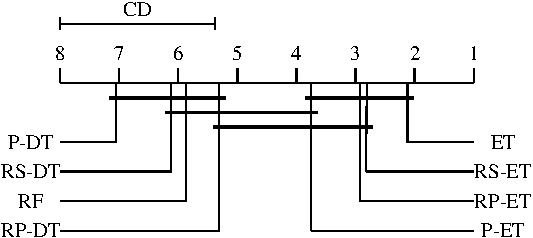
\includegraphics[width=0.9\textwidth]{figures/ch8_rank_small.pdf}
    \caption{Average ranks of all methods.}
    \label{fig:8:small-cmp}
\end{figure}

\begin{table}
    \centering
    \footnotesize
  \begin{tabular}{|l|cccccccc|}
    \hline
         & RF & ET & P-DT & P-ET & RS-DT & RS-ET & RP-DT & RP-ET \\
    \hline
    \hline
        RF     &  ---   & 1/2/13 & 12/4/0  & 1/7/8   & 4/7/5   & 2/2/12 & 1/10/5  & 0/4/12 \\
        ET     &  13/2/1 & ---   & 14/1/1  & 10/5/1  & 13/3/0  & 4/11/1 & 12/2/2  & 5/10/1 \\
        P-DT   &  0/4/12 & 1/1/14 & ---    & 0/4/12  & 2/3/11  & 2/1/13 & 0/4/12  & 0/4/12 \\
        P-ET   &  8/7/1  & 1/5/10 & 12/4/0  & ---    & 9/6/1   & 2/6/8  & 9/6/1   & 0/11/5 \\
        RS-DT  &  5/7/4  & 0/3/13 & 11/3/2  & 1/6/9   & ---    & 0/2/14 & 1/11/4  & 0/4/12 \\
        RS-ET  &  12/2/2 & 1/11/4 & 13/1/2  & 8/6/2   & 14/2/0  & ---   & 11/4/1  & 1/13/2 \\
        RP-DT  &  5/10/1 & 2/2/12 & 12/4/0  & 1/6/9   & 4/11/1  & 1/4/11 & ---    & 0/6/10 \\
        RP-ET  &  12/4/0 & 1/10/5 & 12/4/0  & 5/11/0  & 12/4/0  & 2/13/1 & 10/6/0  & ---\\
    \hline
    \end{tabular}
    \caption{Pairwise t-test comparisons.}
    \label{table:rp:small-ttest}
\end{table}

% ET versus DT

Since all methods are variants of ensembles of decision trees, average
accuracies are not strikingly different from one method to another (see Table 1
of the supplementary materials). Yet, significant trends appear when looking at
Figure \ref{fig:8:small-cmp} and Table \ref{table:rp:small-ttest}.  First, all ET-based
methods are ranked before DT-based methods, including the popular Random
Forest algorithm. Overall, the original ET algorithm is ranked first ($R_{ET} =
2.125$), then come RS-ET and RP-ET at close positions ($R_{RS-ET} = 2.8125$ and
$R_{RP-ET} = 2.9375$) while P-ET is a bit behind ($R_{P-ET} = 3.75$). According
to Figure \ref{fig:8:small-cmp}, only ET is ranked significantly higher than all
DT-based method but looking at Table \ref{table:rp:small-ttest}, the worse ET-based
variant (P-ET) is still 9 times significantly better (w.r.t. the 50
runs over each set) and only 1 times significantly worse than the best DT-based
variant (RP-DT). The separation between these two families of algorithm
thus appears quite significant. This observation clearly suggests that using
random split thresholds, instead of optimized ones like in decision trees, pays
off in terms of generalization.

% RP versus RS et P (ET)

Among ET-based methods, RP-ET is better than P-ET but it is superseded by ET and
RS-ET in terms of average rank. Since RS-ET is a particular case of RP-ET, this
suggests that we are slightly overfitting when tuning the additional parameter
$\alpha_s$. And indeed RP-ET is better ranked than RS-ET in average on the validation
set (results not shown). Table~\ref{table:rp:small-ttest} however indicates
otherwise and makes RP-ET appear as slightly better than RS-ET (2/13/1).
Regarding ET over RP-ET, the better performance of the former (5/10/1) is
probably due to the fact that in ET subsets of features are redrawn locally at
each node when building trees and not once and for all prior to their
construction. This gives less chances to generate improper trees because of a
bad initial choice of features and thus leads to a lower bias and a better
accuracy.

% RP versus RS et P (DT)

Among DT-based methods, RP-DT now comes first (mean rank of 5.3125),
then RF ($R_{RF} = 5.875$), RS-DT ($R_{RS-DT} = 6.125$) and then P-DT
in last ($R_{P-DT} = 7.0625$). RP is only significantly worse than
another DT-based variant on 1 dataset. The extra-randomization brought
by the random choices of both samples and features seems to be
beneficial with decision trees that do not benefit from the
randomization of discretization thresholds. The fact that RF samples
features locally does not appear here anymore as an advantage over RP
(RF is significantly worse on 5 problems and better on only one),
probably because the decrease of bias that it provides does not exceed
the increase of variance with respect to global feature selection.


\section{On Memory}
\label{sec:9:memory}

\section{Conclusions}
\label{sec:9:conclusions}
